

\documentclass[16pt]{article}
\usepackage{graphicx}
\usepackage{array}
\begin{document}



\begin{titlepage}
 
       

       \hfill\hfill\hfill

       {\LARGE{\textbf{e-Yantra Summer Internship-2015 \\ }}}
       
       \vspace{3cm}
       {\Large{\textbf{IoT Connected valves for irrigation of}}} \\  
       % Print the main header
      
       
        {\Large{\textbf{\hspace{3.2cm} greenhouse}}}
        
         \vspace{3cm}
        {\underline{\textbf{Interns:}}} \\
        
        Jayant Solanki \\
        
        Kevin D'souza  
        
        \vspace{1cm}
        
          {\underline{\textbf{Mentors:}}} \\
          
          Ajit Harpude \\
          
          Vishwanathan Iyer
          
\end{titlepage}
\tableofcontents
\vspace{15cm }

\section{Abstract}

 \vspace{0.5cm}
 This project aims to build a copamct and portable module that can be remotely accessed 
 to turn ON/OFF the water supply in a trough, terrace garden or even an agricultural farm. The solution promises to be cheap and afforadble to the common man and 
 the setup is intended to be simple and without hassle. This project aims to touch the lack of automation on irrigation systems in agriculture 
 and thus increase the throuput of the average farmer. 
 
 Once installed this setup would allow you to remotely control the valve for one's irrigation system and also provides additional features such as 
 timing based control and frequency in watering. This could really ease the user of his worry when he/she is not at around the house or the farm. 
 
 Latter part of this project also includes experimentation regarding moisture sensor integration. This would mean effective feedback to the user for 
 watering. The ultimate goal of the project would be to eliminate the user from this loop and provide effective automation in irrigation through the 
 Internet-of-things approach.


\vspace{12cm}

%\begin{tabbing}
%	\hspace{5cm}	
%        \LARGE{INDEX}                % Print the main header
%\end{tabbing}

%\vspace{0.5cm}


%\begin{enumerate}
%\def\labelenumi{\arabic{enumi}.}
%\itemsep1pt\parskip0pt\parsep0pt
%\item 
% Objective and Deliverables
%\item
%  Installation
%\item
%  Literature review 
%\item
%  ESP8266 WiFi module 
%\item
%  Circuit design and testing 
%\item
%  nodeMCU firmware
%\item
%  Protocols for IOT applications and MQTT
%\item
%  MOSCA broker 
%\item 
%  Database handling and UI design 
%\item 
%  Power analysis
%\item 
%  Cost analysis 
%\item 
%  Experimental features and notes 

%\end{enumerate}

%\vspace{11.5cm}


\section{Objective and Deliverables} 

\vspace{1cm}
  {\Large{\textbf{Objective}}} \\
  
  \vspace{0.1cm}
  
  Development of a IOT based low-cost, low-power, standalone module for the automation of Irrigation in a greenhouse.
  
   \vspace{0.6cm}
   
  {\textbf{Deliverables}}
  
\begin{itemize}
\item Demonstration of control of valves remotely
\item Designing a user interfrace for the same 
\item Adding features to the UI 
\item Detailed report on power consumption of the system
\item Exploring experimental features like moisture sensor integration
\item Detailed report of the design process with documented code
\end{itemize}

\vspace{8cm}

\section{Installation}
 
\vspace{1cm}                                    % Print the main header


 
\subsection{Ubuntu}

\hfill
  \begin{enumerate}
  \item
    Have Ubuntu image in pen-drive or a cd
  \item
    Take care to disable secure boot before installation
  \item
    After installation if windows doesn't show in the boot options then
    repair the GRUB from UBUNTU using \emph{boot repair}.Have boot repair in a disc or pen-drive.
  \item
    If you use face further problems use GRUB customizer from UBUNTU.Install Grub customizer from software centre.
  \item
    Once Windows shows in boot options then change the Boot preference
    order from windows by going to the bios setup.
  \item
    In Sony systems while booting use \emph{ASSIST} key
  \end{enumerate}
  
for further information look up this repository 
%www.github.com/
  
\hfill

\subsection{openhab}


Studied openHAB, The thing system and other engines and found that among these openHAB was the best option available, since it was fully open sourced and it
consisted of nearly 100+ addons. It also support MQTT binding which will be useful later on as a minimal size packet data communication protocol.

\hfill

\textbf{Installation of openHAB runtime}

\begin{enumerate}

  \item Download openHAB from its Github repository https://github.com/openhab
  \item Extract the zip file to a suitable directory of your Linux system

  \end{enumerate}
  
\hfill

{\Large\item\textbf{Installatio-of-Apache2-,-PHP-and-MySQL-LAMP-server}} 

\vspace{0.5cm}

{\underline{\Large{About LAMP}}}

  LAMP stack is a group of open source software used to get web servers up
  and running. The acronym stands for Linux, Apache, MySQL, and PHP. Since
  the virtual private server is already running Ubuntu/openSuse, the linux
  part is taken care of. Here is how to install the rest.


  \begin{enumerate}
  

  
%  \begin{center}\rule{3in}{0.4pt}\end{center}

  {\Large{\item{\textbf{Step 1---Install Apache}}}}
  
  \hfill

  To install apache, open terminal and type in these commands: \\
  \textbf{For Ubuntu} \\
  \texttt{sudo apt-get update} 

  \texttt{sudo apt-get install apache2}

  \textbf{For openSuse}

  \texttt{sudo zypper in apache2}

  \textbf{Firewall Adjustments}

  In openSuse, by default the firewall configuration blocks all traffic
  coming on port 80 to your machine. So if you need to allow access so
  that the web server can be accessed from within a LAN we need to fine
  tune the firewall configuration. The below step needs to be performed as
  root user. The supplied configurations are called apache2 and
  apache2-ssl. They can be enabled via YaST, by adding them to
  FW\_CONFIGURATIONS\_EXT in the following path /etc/sysconfig/SuSEfirewall2
  
  \vspace{0.5cm}

  \texttt{sysconf\_addword /etc/sysconfig/SuSEfirewall2 FW\_CONFIGURATIONS\_EXT apache2}
  \texttt{sysconf\_addword /etc/sysconfig/SuSEfirewall2 FW\_CONFIGURATIONS\_EXT apache2-ssl}
  \texttt{rcSuSEfirewall2 restart}
  
   \vspace{0.5cm}

  \textbf{Starting Server}

  Start the server and configure it to automatically start at boot time.

  \texttt{rcapache2 start} \texttt{chkconfig -a apache2}
  
   \vspace{0.5cm}

  {\Large{\item{Step 2---Install MySQL}}}
  
   \vspace{0.5cm}

  MySQL is a powerful database management system used for organizing and
  retrieving data

  To install MySQL, open terminal and type in these commands:

  \textbf{For Ubuntu} \\ sudo apt-get install mysql-server
  libapache2-mod-auth-mysql php5-mysql

  \textbf{For openSuse}

  \texttt{sudo zypper install mysql-server}

  \textbf{To start the server}

  \texttt{sudo systemctl start mysql.service}
  
   \vspace{1cm}

  {\Large{\item{Step 3---Install PHP}}}
   \vspace{0.5cm}

  PHP is an open source web scripting language that is widely use to build
  dynamic webpages.

  To install PHP, open terminal and type in this command.

  \textbf{For Ubuntu}

  \texttt{sudo apt-get install php5 libapache2-mod-php5 php5-mcrypt}

  \textbf{For openSuse}

  \texttt{sudo zypper in php5 php5-mysql apache2-mod\_php5}
  
   \vspace{0.5cm}

  {\underline{\textbf{Installing phpMyAdmin}}}

  \textbf{For Ubuntu}

  \texttt{sudo apt-get install phpMyAdmin}

  \textbf{For OpenSuse}

  \texttt{sudo zypper in phpMyAdmin}
   \vspace{0.5cm}

  Finally restart apache so that all of the changes take effect:

  \textbf{For Ubuntu}

  \texttt{sudo service apache2 restart}

  \textbf{For openSuse}

  \texttt{sudo systemctl start apache2.service}
   \vspace{0.5cm}

  \end{enumerate}

  

{\Large{\item\textbf{Broker and nodejs}}} 
 \vspace{0.5cm}

Based on their use, there are two widely available MQTT brokers
available on the web. 
%* \href{http://mosquitto.org/}{Mosquitto} *
%\href{https://github.com/mcollina/mosca}{Mosca}

We chose Mosca because it is: 

\begin{enumerate}

\item MQTT 3.1 compliant.
\item supporting various storage options for QoS 1 offline packets, and subscriptions.
\item As fast as it is possible.
\item Usable inside ANY other Node.js app.

\end{enumerate}
 \vspace{0.5cm}

{\Large{\textbf{Installation}}}

%\begin{center}\rule{3in}{0.4pt}\end{center}

\textbf{Installation on a OpenSuse system (version
13.1)}

\textbf{Part 1} First install nodejs and npm if both are absent in your
system.

 \vspace{1cm}
 
\textbf{Nodejs}

\begin{quote}
\texttt{sudo zypper install nodejs}
\end{quote}

\textbf{npm}

\begin{quote}
\texttt{sudo zypper install npm}
\end{quote}

If everything goes right (no errors) then proceed to second part.
 \vspace{0.5cm}

\textbf{Part 2}

\textbf{Installation of Mosca}

\begin{quote}
\texttt{npm install mosca}
\end{quote}

If everything goes write then you are good to go.
 \vspace{0.5cm}

\textbf{To start the broker} \textgreater{}\texttt{mosca}

\textbf{Note:} For persistence mode, broker requires mongodb/redis
installed on the system. Installation codes are:
\textgreater{}\texttt{sudo zypper install mongodb-org}

To start the database service
\textgreater{}\texttt{sudo service mongod start}
 \vspace{0.5cm}

%\begin{center}\rule{3in}{0.4pt}\end{center}

\textbf{Installation on an Ubuntu system (version
14.4)}

\textbf{Part 1} First install nodejs and npm if both are absent in your
system.

\textbf{Nodejs}

\begin{quote}
\texttt{sudo apt-get update}
\end{quote}

\begin{quote}
\texttt{sudo apt-get install nodejs}
\end{quote}

\begin{quote}
\texttt{sudo ln -s /usr/bin/nodejs /usr/bin/node}
\end{quote}

\textbf{npm}

\begin{quote}
\texttt{sudo apt-get install npm}
\end{quote}

If everything goes right (no errors) then proceed to second part.

 \vspace{0.3cm}

\textbf{Part 2}

\textbf{Installation of Mosca}

\begin{quote}
\texttt{sudo npm install debug}
\end{quote}

\begin{quote}
\texttt{sudo npm install mosca bunyan -g} //for installing mosca
globally
\end{quote}

\begin{quote}
\texttt{sudo npm install daemon}
\end{quote}



If everything goes write then you are good to go.

 \vspace{0.3cm}

\textbf{To start the broker} \textgreater{}\texttt{mosca}

\textbf{Note:} For persistence mode, broker requires mongodb/redis
installed on the system. Installation codes are:
\textgreater{}\texttt{sudo apt-get update}
\textgreater{}\texttt{sudo apt-get install -y mongodb-org}

To start the database service
\textgreater{}\texttt{sudo service mongod start}

 \vspace{0.5cm}

{\Large{\textbf{Testing the broker}}}

First to test the mqtt broker, we need to install a mqtt client on the
system.

\begin{quote}
\texttt{sudo npm install mqtt -g}
\end{quote}

\textbf{Second, creating scripts for testing}

Script for starting MQTT broker service, \textbf{mosca-app.js}

%\begin{Shaded}
%\begin{Highlighting}[]
%\KeywordTok{var} \NormalTok{mosca = }\FunctionTok{require}\NormalTok{(}\StringTok{'mosca'}\NormalTok{)}

%\KeywordTok{var} \NormalTok{ascoltatore = \{}
 % \CommentTok{//using ascoltatore}
 % \DataTypeTok{type}\NormalTok{: }\StringTok{'mongo'}\NormalTok{,        }
 %\DataTypeTok{url}\NormalTok{: }\StringTok{'mongodb://localhost:27017/mqtt'}\NormalTok{,}
 % \DataTypeTok{pubsubCollection}\NormalTok{: }\StringTok{'ascoltatori'}\NormalTok{,}
 % \DataTypeTok{mongo}\NormalTok{: \{\}}
%\NormalTok{\};}

%\KeywordTok{var} \NormalTok{moscaSettings = \{}
 % \DataTypeTok{port}\NormalTok{: }\DecValTok{1883}\NormalTok{,}
 % \DataTypeTok{backend}\NormalTok{: ascoltatore,}
 % \DataTypeTok{persistence}\NormalTok{: \{}
  %  \DataTypeTok{factory}\NormalTok{: }\OtherTok{mosca}\NormalTok{.}\OtherTok{persistence}\NormalTok{.}\FunctionTok{Mongo}\NormalTok{,}
  %  \DataTypeTok{url}\NormalTok{: }\StringTok{'mongodb://localhost:27017/mqtt'}
 % \NormalTok{\}}
%\NormalTok{\};}

%\KeywordTok{var} \NormalTok{server = }\KeywordTok{new} \OtherTok{mosca}\NormalTok{.}\FunctionTok{Server}\NormalTok{(moscaSettings);}
%\OtherTok{server}\NormalTok{.}\FunctionTok{on}\NormalTok{(}\StringTok{'ready'}\NormalTok{, setup);}

%\OtherTok{server}\NormalTok{.}\FunctionTok{on}\NormalTok{(}\StringTok{'clientConnected'}\NormalTok{, }\KeywordTok{function}\NormalTok{(client) \{}
 %   \OtherTok{console}\NormalTok{.}\FunctionTok{log}\NormalTok{(}\StringTok{'client connected'}\NormalTok{, }\OtherTok{client}\NormalTok{.}\FunctionTok{id}\NormalTok{);     }
%\NormalTok{\});}

%\CommentTok{// fired when a message is received}
%\OtherTok{server}\NormalTok{.}\FunctionTok{on}\NormalTok{(}\StringTok{'published'}\NormalTok{, }\KeywordTok{function}\NormalTok{(packet, client) \{}
 % \OtherTok{console}\NormalTok{.}\FunctionTok{log}\NormalTok{(}\StringTok{'Published'}\NormalTok{, }\OtherTok{packet}\NormalTok{.}\FunctionTok{payload}\NormalTok{);}
%\NormalTok{\});}

%\CommentTok{// fired when the mqtt server is ready}
%\KeywordTok{function} \FunctionTok{setup}\NormalTok{() \{}
 % \OtherTok{console}\NormalTok{.}\FunctionTok{log}\NormalTok{(}\StringTok{'Mosca server is up and running'}\NormalTok{)}
%\NormalTok{\}}
%\end{Highlighting}
%\end{Shaded}

To start the service type \textgreater{}\texttt{node mosca-app.js}

Script for MQTT Publishing Client \textbf{node client-pub.js}

%\begin{Shaded}
%\begin{Highlighting}[]
%\KeywordTok{var} \NormalTok{mqtt    = }\FunctionTok{require}\NormalTok{(}\StringTok{'mqtt'}\NormalTok{);}
%\KeywordTok{var} \NormalTok{client  = }\OtherTok{mqtt}\NormalTok{.}\FunctionTok{connect}\NormalTok{(}\StringTok{'mqtt://localhost'}\NormalTok{);}
 
%\OtherTok{client}\NormalTok{.}\FunctionTok{on}\NormalTok{(}\StringTok{'connect'}\NormalTok{, }\KeywordTok{function} \NormalTok{() \{}
 % \OtherTok{client}\NormalTok{.}\FunctionTok{publish}\NormalTok{(}\StringTok{'presence'}\NormalTok{, }\StringTok{'Hello!'}\NormalTok{, \{}\DataTypeTok{retain}\NormalTok{: }\KeywordTok{false}\NormalTok{, }\DataTypeTok{qa}\NormalTok{: }\DecValTok{1}\NormalTok{\});}
%\OtherTok{client}\NormalTok{.}\FunctionTok{end}\NormalTok{();}
%\NormalTok{\});}
%\end{Highlighting}
%\end{Shaded}

Script for MQTT Publishing Client \textbf{node client-sub.js}

%\begin{Shaded}
%\begin{Highlighting}[]
%\KeywordTok{var} \NormalTok{mqtt    = }\FunctionTok{require}\NormalTok{(}\StringTok{'mqtt'}\NormalTok{);}
%\KeywordTok{var} \NormalTok{client  = }\OtherTok{mqtt}\NormalTok{.}\FunctionTok{connect}\NormalTok{(}\StringTok{'mqtt://localhost'}\NormalTok{);}
 
%\OtherTok{client}\NormalTok{.}\FunctionTok{on}\NormalTok{(}\StringTok{'connect'}\NormalTok{, }\KeywordTok{function} \NormalTok{() \{}
 % \OtherTok{client}\NormalTok{.}\FunctionTok{subscribe}\NormalTok{(}\StringTok{'presence'}\NormalTok{);}
 
%\OtherTok{client}\NormalTok{.}\FunctionTok{on}\NormalTok{(}\StringTok{'message'}\NormalTok{, }\KeywordTok{function} \NormalTok{(topic, message) \{}
 % \OtherTok{console}\NormalTok{.}\FunctionTok{log}\NormalTok{(}\OtherTok{message}\NormalTok{.}\FunctionTok{toString}\NormalTok{());}
%\OtherTok{client}\NormalTok{.}\FunctionTok{end}\NormalTok{();}
 % \NormalTok{\});}
%\NormalTok{\});}
%\end{Highlighting}
%\end{Shaded}

Open a new Terminal and Execute above MQTT Subscription Client
client-sub.js \textgreater{}\texttt{node client-pub.js}

Now open a differnent Terminal and Execute above MQTT Subscription
Client client-pub.js \textgreater{}\texttt{node client-sub.js}

\textbf{Successful Output From client-sub.js terminal}

\begin{quote}
\texttt{Hello!}
\end{quote}

\vspace{0.5cm}

{\Large{\textbf{Troubleshooting}}}

%\begin{center}\rule{3in}{0.4pt}\end{center}

If while installing mosca there are errors in fetching the links from
server, do any of the following 

\begin{itemize}

\item Check that nodejs version is not
`pre', if it is then update it to a stable non pre version.
\item reinstalling nodejs and npm in root mode. 
\item restart your system.

\end{itemize}

While executing those scripts, if any of the nodejs script file shows
error \textbf{Mqtt module not found}, then copy the scripts to a folder
inside mosca directory, and try executing from there.

For \textbf{openSuse} users, open firewall in yast2 GUI. Then go to
allowed service, then go to to advance option, there enter 1883 inside
tcp port.

  
\end{enumerate}


{\LARGE{\textbf{Literature review}}}
\vspace{0.5cm}

\begin{itemize}

{\Large{\item{\textbf{The Thing system - Architecture}}}}

%\begin{center}\rule{3in}{0.4pt}\end{center}

%\begin{figure}[htbp]
%\centering
%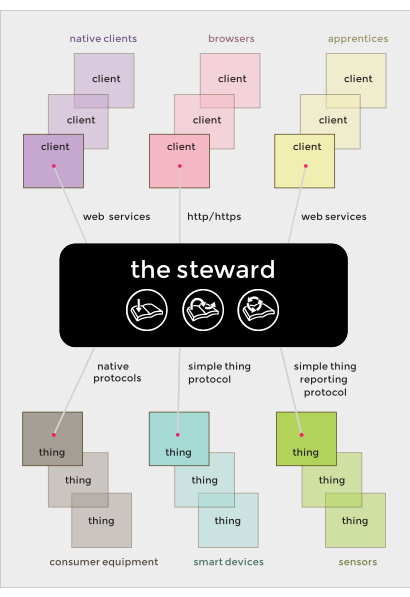
\includegraphics{http://thethingsystem.com/dev/images/thing.architecture.png}
%\end{figure}
\vspace{0.5cm}

The steward is center of the system, monitoring and controlling all
sorts of things, according to the directives it receives from various
clients.
\vspace{0.5cm}

{\Large{\textbf{Communicating with
Things}}}

%\begin{center}\rule{3in}{0.4pt}\end{center}

There are three different protocols that the steward uses to communicate
with a thing. 

\begin{enumerate}


\item With consumer equipment native protocol is used.
\item Things concerned with sensors reading reports uses
%\href{http://thethingsystem.com/dev/Thing-Sensor-Reporting-Protocol.html}{Thing
%Sensor Reporting Protocol}.
%Codes are found on
%\href{https://github.com/TheThingSystem/steward/tree/master/things/examples}{Github}.
\item Things performing some events uses
%\href{http://thethingsystem.com/dev/Simple-Thing-Protocol.html}{Simple Thing Protocol}.

\end{enumerate}

\vspace{0.5cm}

{\Large{\textbf{Communication with
clients}}}

%\begin{center}\rule{3in}{0.4pt}\end{center}

\begin{enumerate}


\item
  Simple clients like platform specific Arduino, Android, iOS and
  platform neutral HTML5. Code can be found on
  %\href{https://github.com/TheThingSystem/steward/tree/master/clients/examples}{Github}.
\item
  Apprentices, they work autonomously.
  
\end{enumerate}

%{\Large{\textbf{Installation}}}

%\begin{center}\rule{3in}{0.4pt}\end{center}

%Visit
%\href{http://thethingsystem.com/dev/Installation.html}{installation
%page}


{\textbf{\item{\Large{Solenoid valves}}}}

\vspace{0.3cm}

  Found a pdf explaining different types of solenoid valves and their
  power consumption.Holding amperes in case of latching Solenoid valves is
  for momentary time of around 20-50 ms reducing power consumption
  significantly. Here's the link %

\vspace{0.3cm}

{\textbf{\item{\Large{Latching solenoid valves}}}}

  Some of the specifications of the latching solenoid valve related to our
  applications are:
  
  \begin{itemize}

  \item
    operates at 6v dc and 650ma
  \item
    will last around 500K cycles
  \item
    operate normally till about 45 degree celcius(ambient temp)
  \item
    operating pressure upto 6 bar
  \end{itemize}
  
\vspace{0.4cm}

  \textbf{Key points to note:}

  \begin{itemize}

  \item
    Power rating varies from about 7 to 11 watts. Considering the duration
    of the pulse this would be a good change from solenoid valves and
    their continuous power consumption.
  \item
    some of the important features and working of latching valves can be
    found at
    
  \item
    Latching solenoid valves specifications matching irrigation
    applications: port size : 3/4'`and G3/8'`\textasciitilde{}G2''
  \item
    2 port direct acting normally closed solenoid valves : model no L2003
    and L2004
  \item
    Availaible online at stores like Indiamart and Alibaba with price
    ranging from 3-8 US dollars per piece
  \end{itemize}

\hfill

{\textbf{\item{\Large{Batteries}}}}

\hfill

Options for Rechargeable batteries we can use :
\hfill
\begin{enumerate}

\item
  lead acid battery
\item
  alkaline batteries
\item
  nickel-cadmium batteries.
\end{enumerate}

\hfill


Alkaline rechargeable batteries would be suitable for our low power
applications. Some of the important features of these batteries are:
\hfill
\begin{itemize}

\item
  They have a life of around 5 years
\item
  They do not self discharge much(0.3\%/month)
\item
  They are compact and Easy to maintain as well.
\item
  They are cheap and easily replaceable
\end{itemize}

\hfill

{\Large{\textbf{Experimentation}}}

\begin{itemize}

\item
  The batteries need to provide a minimum of 6V or higher
\item
  They need to be 2500maH or greater
\item
  should be able to supply a minimum of 650 ma
\item
  Tried with Alkaline rechargeable batteries and Duracell rechargeable
  batteries
\item
  Make sure to use the batteries of the same make together lest one of
  the batteries discharge faster and also discharge the other batteries
  along with it
\end{itemize}

\hfill

{\Large{\item{\textbf{Power consumption}}}}

\begin{enumerate}

 
\item\textbf{Solenoid Valve}

Power rating of each latching solenoid valve
ranges from 7-11 watts.The energy consumed is significantly reduced when
compared to the solenoid valves without latching, as the time duration
of the pulse is very less, around 50ms.

\item\textbf{ESP8266 WIFI module}

A detailed report of its power consumption can be found later in the
wiki

\end{enumerate}

\end{itemize}
\hfill

{\Large{\textbf{Tasks to accomplish}}}

\begin{enumerate}

\item
  Procure the Latching valve and wireless module
\item
  Design the circuit ready for controlling the valves and check its
  working
\item
  Install necessary software and try and interface the wireless module
  with the comp
\item
  Communicate with the valve remotely
\item
  Install openHAB and MQTT broker
\item
  Control the valve using openHAB GUI
\item
  Work on device discovery and persistence
\item
  Make the PCB for the circuit and try to reduce unnecessary components
\item
  A detailed report on the power consumption of the setup
\item
  Make a compact and portable setup
\end{enumerate}


\vspace{5cm}
{\LARGE{\textbf{ESP8266 WiFi module}}}

\vspace{0.5cm}

ESP8266 is a low power WIFI module which is very much suitable for our
irrigation application. Some of the important features of the ESP8266
are:

\begin{itemize}

\item
  Its an ultra low power module which works on 3.3V. This is ideal for
  IoT applications
\item
  It has high on-chip integration
\item
  It has GPIO support for the application devices that you want to
  control
\item
  It has a 32 bit CPU
\item
  It is very small in size
\item
  It is a low cost module
\item
  It can act as a standalone device without the need of any external
  controller
\end{itemize}

{\Large{\textbf{Progress stages and key points}}}

\begin{itemize}

\item
  Installed CCS successfully but later found that this step was unnecessary.you can skip this step.Download CCS from TI website and follow this link for instructions
\item
  A variety of AT commands are mentioned in the link which will be
  useful to send commanda to the ESP from the serial terminal
\item
  The code for ESP8266 can be written in \emph{C} or \emph{python} with
  the help of the SDK which has extensible functions which are useful
\item
  Not much help exists about coding ESP module using \emph{Energia}
\item
  ESP8266 also has MQTT libraries which can be included for its use
\item
  We can use arduino IDE for programming as there is great support for
  Arduino from the ESP community
\item
  All we have to do is flash the code on the ESP using FTDI and we can
  start programming with arduinoIDE
  
\end{itemize}

We chose to go with ESP8266 over CC3200 because the ESP module had all
the functionalities that we needed and was cheaper, lighter and better
for IoT applications.

\vspace{5.5cm}

{\LARGE{\textbf{IDE for ESP8266}}}

\begin{enumerate}

\item
  ESP8266 comes with the NodeMCU firmware loaded and it accepts LUA
  script which can be loaded into the board using ESplorer IDE, but the
  use of this IDE lacks proper documentation.
\item
  Download ESplorer from the website 
\item
  LUA is an embeddable, fast, powerful and light script. This is useful in data
  description and has procedural syntax. It also has some other
  important features like: Automatic memory management and Garbage
  collection
\item
  One other way of loading code into the ESP is using the Arduino
  IDE.This directly loads code into the EEPROM and the NodeMCU firmware
  can be loaded back in the ESP if
  needed
\item Clone
  arduino IDE fro ESP-Arduino Github repository and follow
  the installation procedure
\end{enumerate}

\vspace{0.5cm}

{\Large{\textbf{MQTT in ESP8266}}}

\begin{itemize}

\item
  The ESP8266 community has come up with a MQTT library which can be
  useful to implement MQTT protocol. Go to ESP-mqtt Gitub repository
 
\item
  MQTT can also be implemented using ESP8266 along with Arduino board
  using espduino library. clone from ESP-duino github repository. This is not
  useful to us as it requires Arduino as an external micro-controller
\item
  MQTT functions are already present in the nodeMCU firmware to be used
\item
  while using Arduino IDE and additional library called
  \emph{Pubsubclient} needs to be downloaded and placed in the libraries
  folder. Go to the pubsubclient github repository
 % \href{https://github.com/Imroy/pubsubclient}{pubsubclient}
\end{itemize}

\vspace{0.5cm}

{\Large{\textbf{Troubleshooting}}}

\begin{enumerate}

\item
  After installation of Arduino if an error saying \emph{JAVA exception
  not supported in headless version} pops up then you have to install
  the nonheadless version of JAVA.Installed open-JDK-non-headless
  version and configured to a new java and the installation problem was
  solved. Refer this
 %\href{http://askubuntu.com/questions/26474/unable-to-install-arduino}{forum}
\end{enumerate}


\vspace{3.5cm}

{\LARGE{\textbf{Circuit design and testing}}}

\begin{enumerate}

{\Large{\item{\textbf{The circuit for controlling of ESP8266}}}}

\vspace{0.5cm}

After successfull installation of the forked version of arduino, testing
of ESP8266 is done. The components used are:

\begin{itemize}

\item
  USB to TTL converter
\item
  wires and jumpers
\item
  ESP module
\item
  1k resistors
\end{itemize}

Before you begin:

\begin{enumerate}

\item
  Test the USB to TTL module for its working.
\item
  Rig up the circuit and try loading programs onto the ESP using arduino
  IDE. Test using sample codes.
\end{enumerate}

\textbf{Key points to note while flashing code}

\begin{itemize}

\item
  GPIO 0 is connected to ground
\item
  Take care of the TX-TX and TX-RX connections.The connections might be
  direct or cross coupled depending on the USB to TTL module used.
\item
  The reset of the ESP module and converter are both connected together
  and pulled high
\item
  Take care to set the baud rate right.115200 works just fine.
\item
  choose the ESP board, port connected and set CPU frequency to 80 Mhz
\end{itemize}

\vspace{0.5cm}
{\Large{\textbf{Troubleshooting}}}

\begin{enumerate}

\item
  If esp-sync and esp-comm failed error then recheck the above
  mentioned.
\item
  If port is greyed out then try changing ownership of port by
  \textgreater{}\texttt{sudo chown \$username /dev/ttyUSB}
\end{enumerate}

\vspace{0.5cm}
\textbf{Testing GPIO's and wifi connection}

Some of the key points observed during testing:

\begin{itemize}

\item
  While testing the GPIO pins of the ESP8266, found that the code only
  works if the GPIO 0 pin is removed from ground(Which is required while
  loading code)
\item
  Sample codes like wifiscan are working fine. If The ESP is able to
  connect to the WIFI's present but the webpage hosted the server is not
  acccessing check authentication details
\item
  Since there was authentication hassle with IITB-Guest wifi that we are
  using, we have decided to setup a local server(WAMP) and a wifi
  hotspot on one of our laptop. Our testing code will enable the ESP8266
  to fetch the html page from the local server and display it on the
  console.
  
\end{itemize}

\vspace{0.5cm}

\textbf{Test codes}

\begin{enumerate}

\item
  The wifiWebServer test code was run on the ESP module and a web server
  was successfully hosted on the ESP.The GPIO were controlled through
  the Web server page
\item
  The solenoid test conducted and verified the working of the solenoid
  in the desired fashion
\item
  The solenoid was controlled using the web server hosted on the ESP
\end{enumerate}

\vspace{0.5cm}

{\Large{\item{\textbf{The circuit for controlling the solenoid valves}}} }

Components required:

\begin{itemize}

\item
  L298N Dual H-bridge
\item
  Power supply or battery
\item
  wires and jumpers
\item
  Latching solenoid valve
\item
  Arduino Mega ADK(any microcontroller)
\end{itemize}

\textbf{Steps}

\begin{itemize}

\item
  The GPIO pins of the arduino are controlled and given as input to the
  IN1,IN2 to control direction and EN1 to control the PWM pulse
\item
  The combination of IN1 and IN2 values control the direction of motion
  of the coil.When IN1 is high and IN2 is low the latch opens and when
  the vice versa happens the latch closes
\item
  As the H-bridge works at 12v(given to the coil) therefore the duration
  of the pulse should be around 20ms for optimum working
\item
  LT293 H-bridge driver IC also can be used to test the
  circuit%\href{http://www.ti.com/lit/ds/symlink/l293.pdf}{LT293}
\item
  This is another alternative to the same, Using dual Hbridge driver
  DRV8841
  %\href{http://www.ti.com/lit/an/slva460/slva460.pdf}{Solenoid\_driving}
\end{itemize}

\end{enumerate}

\vspace{19cm}
{\LARGE{\textbf{nodeMCU firmware}}}
\vspace{0.5cm}

Reasons for Switching from Arduino IDE to nodeMCU firmware

\begin{itemize}

\item
  Arduino IDE doesn't provide us the liberty to do tweaks at the basic
  level which is possible through the nodeMCU firmware
\item
  It cant access the sleep modes of the ESP which are important for our
  IoT application
\item
  checkout the nodeMCU API
  %\href{https://github.com/nodemcu/nodemcu-firmware/wiki/nodemcu_api_en}{nodeMCU}
\item
  nodeMCU firmware comes inbuilt with the ESP8266 and it uses LUA script
  which is a fast and powerful script
\item
  Incase you have erased the original firmware then you can reflash it
  by downloading the firmware here
  %\href{https://github.com/nodemcu/nodemcu-firmware/raw/master/pre_build/latest/nodemcu_latest.bin}{firmware}
\item
  It can be flashed through the esptool. Download ESPTOOL here
  %\href{https://github.com/themadinventor/esptool/}{esptool}.
\item
  Follow the instructions given here
 % \href{http://www.whatimade.today/flashing-the-nodemcu-firmware-on-the-esp8266-linux-guide/}{setup}
 
\end{itemize}

\textbf{Installation procedure:}

\begin{itemize}

\item
  Download nodeMCU latest firmware from the link above
\item
  Download ESPTOOL
\item
  Move to the directory containing esptool and execute the following
  command
\end{itemize}

\begin{quote}
\texttt{sudo python esptool.py -{}-port /dev/ttyUSB0  write\_flash 0x00000 The\_Path\_To\_The\_NodeMCU\_Firmware.bin}
\end{quote}

\begin{itemize}

\item
  Make sure you are connected to the right port and change can access
  it. Else change ownership using
\end{itemize}

\begin{quote}
\texttt{Sudo chown \$username /dev/ttyUSB*}
\end{quote}

\textbf{note:} Make sure GPIO 0 is connected to ground while flashing
\vspace{0.5cm}

\textbf{ESPlorer IDE}

\begin{itemize}

\item
  The ESPlorer IDE is a great tool to work with the ESP8266 making the
  loading of code into the ESP an easy task
\item
  Download ESPlorer here
 % \href{http://esp8266.ru/esplorer/\#download}{ESPlorer}
\item
  ESPlorer is a platform that helps you load lua scripts into the ESP.
  follow this for more help
  %\href{http://randomnerdtutorials.com/esp8266-web-server/}{webserver\_example}
\item
  For the GPIO mapping refer this
  %\href{https://github.com/nodemcu/nodemcu-firmware}{gpio\_map}
\item
  Refer this for some more documentation regarding nodeMCU
  %\href{http://www.nodemcu.com/docs/}{nodeMCU}
\end{itemize}

\textbf{Troubleshooting}

\begin{itemize}

\item
  ESPlorer needs JAVA 7 or higher. install JAVA 8 for ubuntu by
  following these steps
  %\href{http://tecadmin.net/install-oracle-java-8-jdk-8-ubuntu-via-ppa/}{JAVA 8}.
  After downloading ESPlorer make your way to the folder in which
  ESPlorer.jar exists and run this command in the terminal
  \textgreater{}\texttt{java -jar ESPlorer.jar} and your done
\item
  esptool depends on %\href{http://pyserial.sourceforge.net/}{pySerial}
  for serial communication with the target device.
\end{itemize}

If you choose to install esptool system-wide by running
\texttt{python setup.py install}, then this will be taken care of
automatically.
If not using \texttt{setup.py}, then you'll have to install pySerial
manually by running something like \\

\texttt{pip install pyserial},
\texttt{easy\_install pyserial} or
\texttt{apt-get install python-serial} \\
\vspace{0.3cm}
depending on your platform. The
official pySerial installation instructions are
%\href{http://pyserial.sourceforge.net/pyserial.html\#installation}{here}).
This utility actually have a user interface! It uses
%\href{https://docs.python.org/dev/library/argparse.html}{Argparse}
and is rather self-documenting. Try running \texttt{esptool -h}. Or hack the
script to your hearts content. The serial port is selected using the
\texttt{-p} option, like \texttt{-p /dev/ttyUSB0} (on unixen like Linux
and OSX) or \texttt{-p COM1} (on Windows). The perhaps not so obvious
corner case here is when you run esptool in Cygwin on Windows, where you
have to convert the Windows-style name into an Unix-style path
(\texttt{COM1} -\textgreater{} \texttt{/dev/ttyS0}, and so on).

\vspace{9cm}


{\LARGE{\textbf{Protocols for communication}}}

\vspace{0.5cm}

The Protocols that can be looked into are:

\begin{itemize}

\item
  MQTT
\item
  MQTT-SN
\item
  The skinny call control protocol(SCCP)
\item
  6LOWPAN
\item
  LoRaWAN
\item
  Constrained application protocol(COAP)
\item
  Light-weight M2M(LWM2M)
\item
  The simple thing protocol
\end{itemize}

\textbf{Material for reading}

\begin{enumerate}

\item
  Here is a Pdf explaining the LWM2M protocol. This is a very specific
  M2M protocol for Internet of things
  applications.%\href{http://archive.ericsson.net/service/internet/picov/get?DocNo=1/28701-FGB101973}{LWM2M}.
  This protocol intergrates COAP in it as well
\item
  COAP protocol is widely used in IOT applications. Ideal for low power
  and constrained memory usage applications
  %\href{https://tools.ietf.org/html/draft-arkko-core-sleepy-sensors-01}{COAP}.
  This could make use of sleep-wakeup model as mentioned in the pdf
\item
  MQTT-SN is also a very lightweight sensor application protocol.
  MQTT-SN protocol is just an extension of this protocol where the
  communication of sensors and actuators is given importance.There are
  certain changes here and there which would be ideal for sensor
  communication
\item
  Additional features of MQTT-SN are explained here
 %\href{http://mqtt.org/new/wp-content/uploads/2009/06/MQTT-SN_spec_v1.2.pdf}{MQTT-SN}
\item
  Comparison and Pros and cons of MQTT and COAP at the application layer
  %\href{http://www.eclipse.org/community/eclipse_newsletter/2014/february/article2.php}{comparison}
\end{enumerate}

\vspace{0.5cm}

{\LARGE{\textbf{Message queing telemetry transport}}}

\vspace{0.5cm}
Some of the important features of MQTT protocol:

\begin{itemize}

\item
  Its a low power protocol which is useful in IoT applications
\item
  Its a low bandwidth protocol
\item
  Even though its unreliable because it doesn't error checking overheads
  this makes it very lightweight
\item
  It offers three different qualites of service(QOS)
\item
  It is a publish/subscribe model which is ideal for our irrigations
  application
\item
  ESP8266 has inbuilt support for MQTT with all the important functions
\item
  MQTT protocol is explained in detail here
  %\href{http://mosquitto.org/man/mqtt-7.html}{MQTT}
\item
  Look through MQTT as a protocol and its API documentation
  %\href{http://knolleary.net/arduino-client-for-mqtt/api/}{API\_documentation}
\item
  It runs on UDP therefore doesn't need to maintain the connection
  information
\item
  Simple to use
\item
  Less processing at both ends
\end{itemize}

These are the reasons we decided to go with MQTT protocol for our
application.

\vspace{13cm}

{\LARGE{\textbf{MOSCA broker}}}

\vspace{0.5cm}

After successfully installing MOSCA broker on the system, you are now
good to go on next step.

\vspace{0.5cm}
{\Large{\textbf{Running MOSCA}}}

%\begin{center}\rule{3in}{0.4pt}\end{center}

{\textbf{Configuring IP on which MOSCA has to be run.}}

\emph{on the terminal type \textgreater{}\texttt{mosca -help}, it will
display all the handles which mosca currently supports we are going to
use handles, {\textbf{-v, --host, \textbar{} bunyan}}}. \emph{To start the server,on
the terminal type \textgreater{}\texttt{mosca -v --host 'ur ip'
\textbar{}bunyan}}. \\ Server testing can be done via two codes included in
the mosca folder.

\vspace{0.3cm}

\textbf{NOTE}: for opensuse users, make sure that entry for tcp port
1883 is in the firewall for inbound connection.

\begin{itemize}

\item
  to run the code, first run client-sub.js on a diiferent terminal, and
  then run client-pub.js on a second terminal.
\item
  message from the topic subscribed will be printed where client-sub.js
  has been run.
\end{itemize}

\vspace{0.5cm}

{\LARGE{\textbf{Interfacing MOSCA and ESP}}}

\begin{itemize}

\item
  Install MOSCA on your system
\item
  Setup the server using \emph{mosca -v --host \$hostname \textbar{}
  bunyan}
\item
  Burn the LUA scripts on the ESP8266
\item
  send subscribe request from your terminal using
  \textgreater{}\texttt{node client-sub.js} (go to the apprpriate folder
  first)
\item
  send publish command from the terminal
  \textgreater{}\texttt{node client-pub.js}
\item
  see the sent data on your terminal with confirm message
\end{itemize}



{\Large{\textbf{Troubleshooting}}}

\begin{itemize}
\item{\textbf{ESP8266}}

\begin{itemize}

\item
  take care to use the delays at appropriate places so as to send out
  publish and subscribe requests
\item
  LUA syntax must be kept in mind.
\item
  Use \textgreater{}\texttt{tmr.alarm} instead of
  \textgreater{}\texttt{tmr.delay} wherever possible
\end{itemize}

\vspace{0.6cm}

\item{\textbf{MOSCA server}}

\begin{itemize}

\item
  The local IP must be changed in the the ESP and also the
  \textgreater{}\texttt{client-pub.js} and
  \textgreater{}\texttt{client-sub.js} scrits
\item
  The topic must be the same in the \textgreater{}\texttt{client-pub.js}
  and subscribe code in the ESP
\end{itemize}

\vspace{0.5cm}
\end{itemize}

{\Large{\textbf{Configuring MOSCA with
openHAB}}}

%\begin{center}\rule{3in}{0.4pt}\end{center}

After successfully running mosca on the system, it is time to start
running openHAB.

\begin{itemize}

\item
  copy required addons (mqtt binding, mqtt-transport binding,
  persistence binding etc) from the addon zip downloaded from the
  %\href{openHAB}{https://bintray.com/artifact/download/openhab/bin/distribution-1.7.0-addons.zip}
  link to the openhab\textgreater{} addon folder of your system.
\item
  create openhab.cfg from openhab-default.cfg file and add following
  details
\item
  under mqtt transport section update following lines
\end{itemize}

\texttt{javacript       mqtt:broker.url=tcp://192.168.0.100:1883       mqtt:broker.clientId=openhab}

\begin{itemize}


\item your system is now ready for openHAB to start and test a demo site for
glowing a led on esp8266 module.
\item copy content of the folders to the
respective folder in the openHAB 
\item Open browser and type
\textgreater{}\texttt{localhost:8080/openhab.app?sitemap=test}
\item toggle
the switch and you can see led going on and off.

\end{itemize}

\vspace{8cm}

{\LARGE{\textbf{Database handling and UI design\\}}}

\vspace{0.3cm}
{\Large{\underline{\textbf{Table Description}}}}
\vspace{0.2cm}

\textbf{Database name: iot}

Tables in database: 

\begin{itemize}

\item devices
\item groups 
\item sensors
\item tasks  

\end{itemize}

\textbf{Device table}

\textbf{Name:} device

\textbf{\textbar{} Field \textbar{} Type \textbar{} Null \textbar{} Key
\textbar{} Default \textbar{} Extra \textbar{}}

\textbar{} id \textbar{} int(255) \textbar{} NO \textbar{} PRI
\textbar{} NULL \textbar{} auto\_increment \textbar{}

\textbar{} name \textbar{} varchar(255) \textbar{} YES \textbar{}
\textbar{} NULL \textbar{} \textbar{}

\textbar{} macid \textbar{} varchar(30) \textbar{} NO \textbar{}
\textbar{} NULL \textbar{} \textbar{}\\ \textbar{} group \textbar{}
varchar(255) \textbar{} YES \textbar{} \textbar{} NULL \textbar{}
\textbar{}\\ \textbar{} status \textbar{} int(1) \textbar{} YES
\textbar{} \textbar{} NULL \textbar{} \textbar{}\\ \textbar{} battery
\textbar{} varchar(10) \textbar{} YES \textbar{} \textbar{} NULL
\textbar{} \textbar{}\\ \textbar{} seen \textbar{} timestamp \textbar{}
NO \textbar{} \textbar{} CURRENT\_TIMESTAMP \textbar{} on update
CURRENT\_TIMESTAMP \textbar{}\\ \textbar{} action \textbar{} int(1)
\textbar{} YES \textbar{} \textbar{} NULL \textbar{} \textbar{}\\
\textbar{} type \textbar{} varchar(255) \textbar{} YES \textbar{}
\textbar{} NULL \textbar{} \textbar{}

\textbf{Group Table}

\textbf{Name:} groups

\textbf{\textbar{} Field \textbar{} Type \textbar{} Null \textbar{} Key
\textbar{} Default \textbar{} Extra \textbar{}}

id \textbar{} int(10) \textbar{} NO \textbar{} PRI \textbar{} NULL
\textbar{} auto\_increment \textbar{}

name \textbar{} varchar(255) \textbar{} NO \textbar{} \textbar{} NULL
\textbar{} \textbar{}

\textbf{Sensor Table}

\textbf{Name:} sensors

\textbf{\textbar{} Field \textbar{} Type \textbar{} Null \textbar{} Key
\textbar{} Default \textbar{} Extra \textbar{}}

id \textbar{} int(255) \textbar{} NO \textbar{} PRI \textbar{} NULL
\textbar{} auto\_increment \textbar{}

name \textbar{} varchar(255) \textbar{} NO \textbar{} \textbar{} NULL
\textbar{}

\textbf{Tasks Table}

\textbf{Name:} tasks

\textbf{\textbar{} Field \textbar{} Type \textbar{} Null \textbar{} Key
\textbar{} Default \textbar{} Extra \textbar{}}

id \textbar{} int(255) \textbar{} NO \textbar{} PRI \textbar{} NULL
\textbar{} auto\_increment \textbar{}

item \textbar{} varchar(25) \textbar{} NO \textbar{} \textbar{} NULL
\textbar{} \textbar{}

start \textbar{} int(4) \textbar{} YES \textbar{} \textbar{} NULL
\textbar{} \textbar{}

stop \textbar{} int(4) \textbar{} YES \textbar{} \textbar{} NULL
\textbar{} \textbar{}

action \textbar{} int(1) \textbar{} YES \textbar{} \textbar{} NULL
\textbar{}

%\begin{center}\rule{3in}{0.4pt}\end{center}

\textbf{Library used}

Uses php library \textbf{SSKAJE MQTT} for communicating with MOSCA
broker.

%\href{https://sskaje.me}{SSKAJE MQTT}

%\href{https://github.com/sskaje/mqtt}{GITHUB}

\textbf{About the website}

After studying different home automation server, we found that, we need
to create an engine, which will work in the background performing
following automated tasks:

\begin{enumerate}

\item Device discovery \textbf{--\textgreater{}}
\texttt{subscribe.php}
\item Valve and other sensors scheduling
\textbf{--\textgreater{}} \texttt{tasks.php} 
\item Listening for battery status \textbf{--\textgreater{}} \texttt{battery.php} 
\item Listening for Moisture value \textbf{--\textgreater{}} \texttt{moisture.php}

\end{enumerate}


Tasks.php is executed every minute using cron and above other files are
run continuously in php cli mode.

\vspace{13cm}

{\LARGE{\textbf{Power Analysis}}}
\vspace{0.5cm}

{\Large{\textbf{ESP8266}}}

\vspace{0.2cm}

\textbf{Modes of operation of
ESP8266:}

\begin{itemize}

\item
  Active mode : Consumes a peak current of about 200ma. The power
  consumption would be 0.7W
\end{itemize}

The high speed clock is operational and sent to each block enabled by
the clock control register. Lower level clock gating is implemented at
the block level, including the CPU, which can be gated off using the
\emph{WAITI} instruction, while the system is on.

\begin{itemize}

\item
  Sleep mode : consumes about 0.9ma typically and the power consumption
  would be around 3mW
\end{itemize}

Only the RTC is operating. The crystal oscillator is disabled. Any
wakeup events (MAC, host, RTC timer,external interrupts) will put the
chip into the WAKEUP state.

\begin{itemize}

\item
  Wakeup mode : consumes a peak current of 60 ma during wakeup.
\end{itemize}

In this state, the system goes from the sleep states to the PWR state.
Thecrystal oscillator and PLLs are enabled.

\begin{itemize}

\item
  Deep-sleep mode : consumes about 1ma and about 8uW of power in this
  mode
\end{itemize}

Only RTC is powered on --the rest of the chip is powered off. Recovery
memory of RTC can keep basic Wi-Fi connecting information.To be able to implement deep sleep (without adding extra hardware to
generate a wake-up signal), you need to link the \emph{RESET pin to the
GPIO 16 pin}.By linking these, you lose the ability to use GPIO16, but
gain an automatic wake-up from deep sleep after the number of
microseconds that you specify in the \texttt{node.dsleep(time\_in\_us)}
call.It does not require Wi-Fi connection to be maintained. It's mainly for
application with long time lags between data transmission.ESP8266 needs to be waked up by GPIO16 or by other gpio of external MCU.
Thus, GPIO 16 or external GPIO should be connected to RST pin.

\begin{itemize}

\item
  \textbf{\emph{note 1}} : During flashing : consumes a peak current of 75
  ma
\item
  \textbf{\emph{note 2}} : When the ESP wakes from sleep it runs init.lua file again
\end{itemize}

\vspace{0.5cm}
{\Large{\textbf{WIFI sleep modes}}}

\vspace{0.5cm}
{\underline{\texttt{\textbf{wifi.sleeptype()}}}}


\vspace{0.1cm}
  Configures the sleep type for wifi modem


\textbf{\emph{Note}}: works only in wifi.STATION mode

\begin{itemize}

\item
  \textbf{\emph{syntax}}: type\_actual = wifi.sleeptype(type\_need)
\end{itemize}

  \textbf{parameters:}

\begin{itemize}
\item
  \textbf{\emph{wifi.NONE\_SLEEP}}: wake up device from LIGHT\_SLEEP or MODEM\_SLEEP
  mode
\item
  \textbf{\emph{wifi.MODEM\_SLEEP}}: closes wifi modem, but CPU and other peripherals
  still work.
\end{itemize}

It saves power to shut down the Wi-Fi Modem circuit while maintaining a
Wi-Fi connection with no data transmission. It requires the CPU to be
working, as in PWM or I2C applications.

\begin{itemize}

\item
  \textbf{\emph{wifi.LGIHT\_SLEEP}}: close wifi modem, Oscillator and PLL, CPU and
  peripheral enters ``clock-pause'' status.
\end{itemize}

The CPU may be suspended in applications like Wi-Fi switch. Without data
transmission, the Wi-Fi Modem circuit can be turned off and CPU
suspended to save power.

\vspace{0.2cm}

\textbf{\emph{Note 1}}: Both are automatically added by underlying, which
can sleep and be waked up automatically. There is no need of any
processing in hardware.Both can adjust themselves to support the type of
DTIM according to the AP that connected.

\vspace{0.1cm}

\textbf{\emph{Note 2}}: Power saving modes can only be enabled in station
mode

\vspace{0.6cm}

{\Large{\textbf{Implementaton}}}

\vspace{0.3cm}

{\underline{\texttt{\textbf{node.dsleep()}}}}

\vspace{0.3cm}

\textbf{\emph{Description}}: Enter deep sleep mode, wake up when timed out.

\textbf{\emph{Syntax}}: node.dsleep(us, option)

\textbf{\emph{Note}}: This function can only be used in the condition that
esp8266 RST and GPIO16 are connected together. Using sleep(0) will set
no wake up timer, connect a GPIO to pin RST, the chip will wake up by a
falling-edge on pin RST.

option=0, init data byte 108 is valuable; option\textgreater{}0, init
data byte 108 is valueless.

More details as follows: 
\begin{itemize}
\item 0, RF\_CAL or not after deep-sleep wake up, depends on init data byte 108
\item 1, RF\_CAL after deep-sleep wake up, there will belarge current
\item 2, no RF\_CAL after deep-sleep wake up, there will only be small current 
\item 4, disable RF after deep-sleep wakeup, just like modem sleep, there will be the smallest current.
\end{itemize}

\textbf{Parameters}:

\begin{itemize}

\item
  \textbf{us}: number(Integer) or nil, sleep time in micro second. If us
  = 0, it will sleep forever. If us = nil, will not set sleep time.
\item
  \textbf{option}: number(Integer) or nil. If option = nil, it will use
  last alive setting as default option.
\end{itemize}

\textbf{Returns}

\begin{itemize}

\item
  nil
\end{itemize}

\textbf{Example}
\vspace{0.1cm}

--do nothing\\
\texttt{node.dsleep()}\\

\vspace{0.1cm}

--sleep microcesonds\\
\texttt{node.dsleep(1000000)}\\

\vspace{0.1cm}

--set sleep option, then sleep microseconds\\
\texttt{node.dsleep(1000000, 4)}\\

\vspace{0.1cm}

--set sleep option only\\
\texttt{node.dsleep(nil,4)}

\vspace{0.3cm}

\textbf{Note}: \texttt{node.dsleep(0)} makes the ESP sleep forever until
the RST pin is brought low


\vspace{0.5cm}
{\Large{\textbf{Steps}}}

\begin{itemize}

\item
  Connect the GPIO 16 to ground and connect the multimeter in series
  with the battery powering the module
\item
  Change the setting of the multimeter to read current
\item
  Add this line of code in your program
\end{itemize}

\texttt{node.dsleep(time\_in\_us)}

\begin{itemize}

\item
  After this you must see the version of NodeMCU firmware on your screen
  and the init.lua file running again
\item
  If not there might be a problem with the hardware reset and other
  options have to be sought
\end{itemize}

\textbf{WiFi sleep modes}

\begin{itemize}

\item
  Checked using the functions given above in different WiFi sleep modes,
  But could not see any significant change in the current drawn
\item
  The current consumed in Light\_Sleep mode stays to be around 70 ma and
  in Modem\_Sleep to be aroun\vspace{0.5cm}d 80 ma
\item
  The deep sleep is a better option when occasional reception of data is
  required as it can go down to as low as 1 ma, maybe even to
  micro-amperes in some cases, but the problem of the hardware reset is
  yet to be rectified.
\item
  When the ESP looses its connection with the network, it continuously
  scans for any available network and in the process consumes a lot of
  current. Hence it is meaningful to give the ESP a finite number of
  tries to connect and then just make it go to deepsleep mode.
\end{itemize}


\vspace{0.5cm}
{\Large{\textbf{Graphs showing current
consumption}}}

\begin{itemize}

\item
  Average current consumption of the ESP8266 module during its various
  operations over time.Refer figure 1 


\begin{figure}
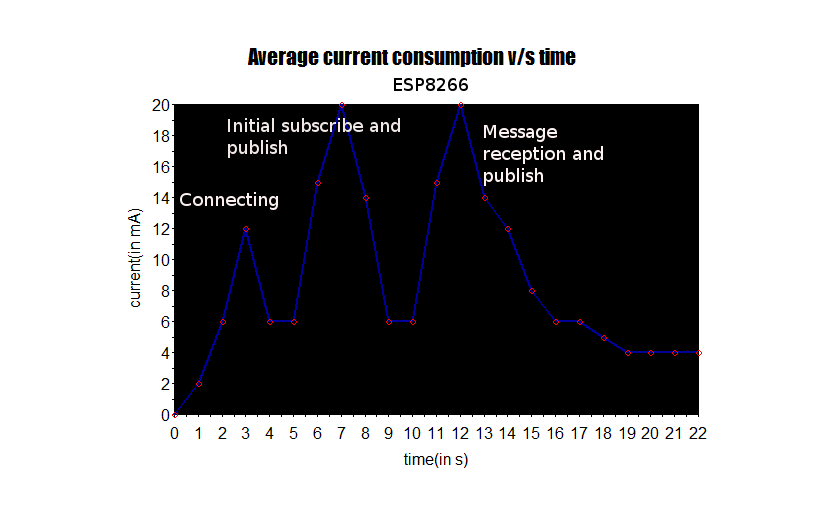
\includegraphics[width=1.2\textwidth]{/home/kevin/git_IoT_WiKi/eYSIP_2015_IoT-Connected-valves-for-irrigation-of-greenhouse.wiki/images/average_current1.png}
\caption{Average}
\end{figure}


\item
  Peak current consumption of the ESP8266 module during its various
  operations over time.Refer figure 2 

\begin{figure}
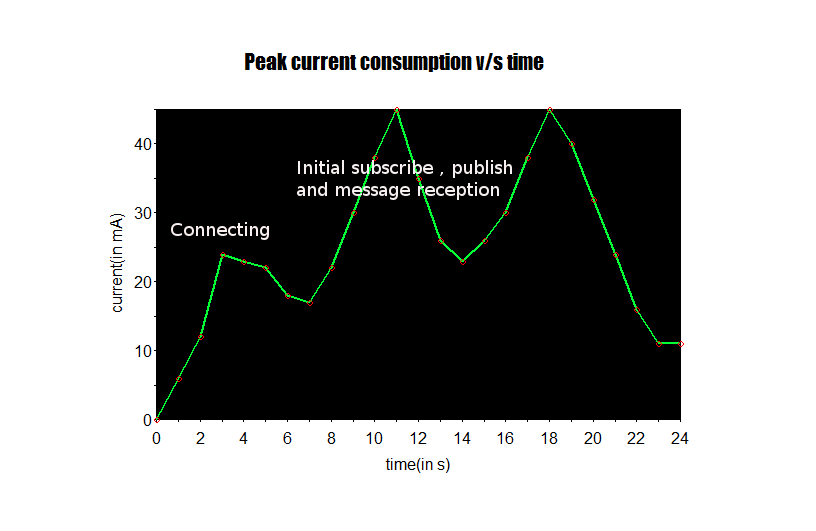
\includegraphics[width=1.2\textwidth]{/home/kevin/git_IoT_WiKi/eYSIP_2015_IoT-Connected-valves-for-irrigation-of-greenhouse.wiki/images/peak_current1.png}
\caption{Peak}
\textbf{Key Points}

  \begin{itemize}

  \item
    The current consumption peaks during message reception and publish
    time
  \item
    The H-bridge consumes more current to turn the latch on than when
    turning it off
  \item
    Overall current peaks up to 45mA at an average
  \item
    The peak current has a possibility to spike up to 75mA
  \item
    There is a wide fluctuation in the current being drawn even during
    idle time therefore there is a possibility that the battery might
    drain out if the power is not switched off at regular intervals
  \end{itemize}
\end{figure}

  
\item
  A graph showing the breakup between the average current consumed by
  the H-bridge(theoretical) and the ESP8266 module.Refer figure 3
\end{itemize}

\begin{figure}
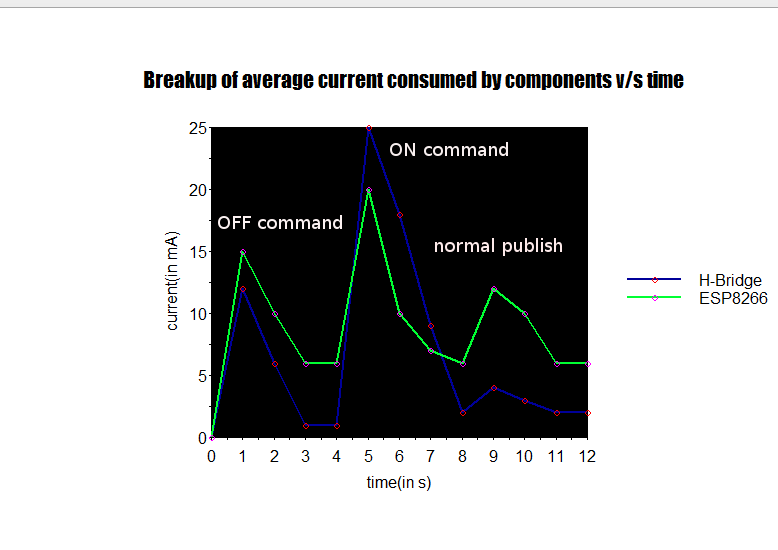
\includegraphics[width=1.2\textwidth]{/home/kevin/git_IoT_WiKi/eYSIP_2015_IoT-Connected-valves-for-irrigation-of-greenhouse.wiki/images/breakup1.png}
\caption{Breakup}
\end{figure}
  
{\Large{\textbf{Observations}}}

\begin{itemize}

\item
  At idle we can observe an average current of about 20mA
\item
  A 2500 mA will last for a maximum of 4 days
\item
  The sleep option of the ESP have to be tapped and as the \\
  \texttt{node.dsleep()} function is not working the options we can look
  into are:
\end{itemize}

\begin{enumerate}

\item
  Use a cheap external controller to wake the ESP8266
\item
  Change the ESP8266 firmware to one of the SDK versions
\item
  Wait for an update to the nodeMCU firmware
\end{enumerate}

\vspace{0.5cm}
\textbf{Troubleshooting}

\begin{itemize}
\item
  Even after connecting the GPIO 16 pin to the RESET pin the ESP doesn't
  wake up to its initial state. It wakes up to some random condition and
  halts the ongoing process
\item
  The ESP8266 has bugs with its software RESET. Therefore an external
  controller might be required to pull its reset pin low if one wants to
  explore the sleep modes of ESP
\end{itemize}

Follow this link for additional info
%\href{http://tinker.yeoman.com.au/2015/03/08/reducing-esp8266-power-consumption-using-deep-sleep/}{Sleep}

\vspace{0.5cm}
{\Large{\textbf{Future plans}}}

\vspace{0.3cm}
In the future we could try to integrate solar power into the module. The
Valve would still be driven by the battery but the ESP8266 module could
be driven by Solar cells during the day and charge the battery during
the night.

\vspace{0.3cm}

\textbf{Problems}

\begin{itemize}

\item
  The amount of current a solar cell can give is very less, about 40ma
\item
  The ESP module requires a minimum of 350 ma. So it would take many
  such cells to give power to the ESP which would in-turn turn out to be
  costly.
\end{itemize}

\vspace{10.5cm}

{\LARGE{\textbf{Cost analysis}}}

\vspace{19cm}
{\LARGE{\textbf{Experimental features and notes}}}

\vspace{0.5cm}

\begin{itemize}

\item{\textbf{YL-69 Soil Hygrometer Humidity \& Soil Moisture Detection Sensor}}

%\begin{figure}
%\centering
%\includegraphics{http://www.tiagoespinha.net/wp-content/uploads/2014/05/2014-05-09-12.51.20.jpg}
%\caption{YL - 69 moisture sensor}
%\end{figure}

\vspace{0.3cm}
This is an Electrical resistance Sensor. The sensor is made up of two
electrodes. This soil moisture sensor reads the moisture content around
it. A current is passed across the electrodes through the soil and the
resistance to the current in the soil determines the soil moisture. If
the soil has more water resistance will be low and thus more current
will pass through. On the other hand when the soil moisture is low the
sensor module outputs a high level of resistance. This sensor has both
digital and analogue outputs. Digital output is simple to use but is not
as accurate as the analogue output.

\vspace{0.5cm}

{\Large{\textbf{Specifications}}}

\begin{itemize}

\item
  Vcc power supply : 3.3V or 5V
\item
  Current : 35mA
\item
  Signal output voltage : 0-4.2V
\item
  Digital Outputs : 0 or 1
\item
  Analog : Resistance (Ω)
\item
  Panel Dimension : 3.0cm by 1.6cm
\item
  Probe Dimension : 6.0cm by 3.0cm
\item
  GND : Connected to ground
\end{itemize}

\vspace{0.5cm}
{\Large{\textbf{Key Features}}}

\begin{itemize}

\item
  The sensor comes with a small PCB board fitted with LM393 comparator
  chip and a digital potentiometer.
\item
  Digipots are used mostly in scaling analog signals to be used in a
  microcontroller.
\item
  Digipot output resistance is variable based on digital inputs and thus
  also know as resistive digital-to-analog converters (RDACs).
\item
  Available for cheap (Rs. 150)
\item
  Efficient in power savings as works on 3.3 volts
\item
  Operates on a range of voltages so that the wrong voltage wont spoil
  the sensor
\item
  Not bulky but light and slender, which is an advantage for many
  applications
\item
  Soil moisture module is most sensitive to the ambient humidity is
  generally used to detect the \vspace{0.5cm}moisture content of the soil
\end{itemize}

{\Large{\textbf{Implementation}}}

\begin{itemize}

\item
  Make the PCB which encompasses the ESP module, YL-69 moisture sensor
  and the YL-69 PCB
\item
  Continuously powering the sensor module will corrode the moisture
  sensor overtime. Therefore control the power to the moisture sensor
  using a GPIO pin of ESP8266
\item
  The Analog out pin A0 of the sensor module is connected to the ADC pin
  of ESP8266
\item
  The signal voltage range is 0 - 4.2V and this has to be brought to 0 -
  1.2v. Voltage divider with 1K and 3K are used for the same
\item
  Make sure to keep common grounds
\item
  The Digital out D0 can also be used to check whether the moisture
  reaches beyond a certain threshold
\item
  After the installation check the values that the sensor gives for dry,
  wet and humid soil and process accordingly
\end{itemize}

\vspace{0.5cm}

{\Large{\item{\textbf{Schematic and PCB
Design}}}}

\end{itemize}

{\textbf{Schematics in KICAD}} \\
Install KICAD from the ubntu software centre along with the additional
addons and tools.

Here is a tutorial that will guide you in the making of schematics using
%\href{https://www.youtube.com/watch?v=rkQ0nVX1q1k}{KICAD}

\begin{itemize}

\item
  If you want to delete, add or functionally change a component, it's
  best to change the schematic and repeat the entire process again
\item
  Make changes in EESCHEMA, re-annotating the components if necessary
  \vspace{0.2cm}
\end{itemize}

{\textbf{Netlists and
footprints}}

\begin{itemize}

\item
  After completing the schematic, generate a netlist that contains all
  the components and their connections
\item
  Save netlist in EESCHEMA (schematic editor)
\item
  After generating the netlist associate footprints in CVPCB
\item
  Each component has its own footprint to be associated to it
\item
  After associating all the components to their respective footprints
  load the netlist in PCBNEW (backup the .brd first!)
%\item
 % A tutorial
 % \href{http://store.curiousinventor.com/guides/kicad/schematic_to_layout}{design}
\end{itemize}

%Here is a tutorial to generate a netlist and associate footprints
%\href{https://www.youtube.com/watch?v=8HNMihqa844}{Tutorial}

\begin{itemize}

\item
  Sometimes the required footprints are not available in KICAD but you
  can make your own footprints in CVPCB
%\item
%  Here's a link to the same
%  \href{http://kicadhowto.wikidot.com/mcf1foot1}{footprints}
%\item
%  Here's a video tutorial explaining how to make your own footprint
%  \href{https://www.youtube.com/watch?v=aVNMJVaRf6M}{video}
\end{itemize}

{\textbf{PCB designing with
PCBNEW}}

Here is a list of tutorials for PCB making

%\begin{itemize}

%\item
%  \href{http://store.curiousinventor.com/guides/kicad/pcb_layout/change_part/}{PCB}
%\item
%  \href{http://kicadhowto.wikidot.com/}{How \_to}
%\item
 % \href{http://store.curiousinventor.com/guides/kicad/pcb_layout/}{PCB
%  making}
%\item
%  \href{https://www.youtube.com/watch?v=TYqmmj6SO-k}{video}
%\end{itemize}
\vspace{17cm}

{\LARGE{\textbf{Cost analysis}}}

\vspace{1cm}
\begin{tabular}{|m{5cm}|m{3.5cm}|}
	\hline
	{\bf Items} & {\bf Est. cost in Rupees}\\ \hline
	ESP8266 & 400 \\ \hline
	Rechargible Alkaline battery & 150 \\ \hline
	H-bridge & 100 \\ \hline 
	Latching Solenoid valve & 430 \\ \hline
	Total cost & 1080 \\ \hline 
\end{tabular} 

\vspace{15cm}
{\LARGE{\textbf{Bugs}}}


\vspace{19cm}
{\LARGE{\textbf{Future work}}}

\end{document}

